\subsection{%
  Определение, примеры
}
\begin{definition}
	Множество $V$, с операциями $+, \times\lambda \,\,(\lambda \in \RR(\CC))$, называется ЛП (над полем $\RR(\CC)$), если
	\begin{axi}[1]
		\hspace{0.5em}1) - 4) аббелева аддитивная \hyperref[def:group]{группа}.
	\end{axi}
	\begin{axi}[2]
		\hspace{0.5em}5) $\exists \mathbbold{1}_{\RR(\CC)} \mid \mathbbold{1} \times x = x \,\,\,\, \forall x \in V$\\[1.5mm]
		\hspace*{3.3em}6) $\lambda(\mu x) = (\lambda\mu)x; \,\, \lambda, \mu \in \RR (\CC);\,\, x \in V$\\[1.5mm]
		\hspace*{3.3em}7) $(\lambda + \mu) \times x = \lambda x + \mu x$\\[1.5mm]
		\hspace*{3.3em}8) $\lambda(x + y) = \lambda x + \lambda y; \,\, x, y \in V$\\
	\end{axi}
\end{definition}
\textbf{Модели (содержательные)}
\begin{enumerate}
	\item Пространство геометрических векторов (точнее --- направленных отрезков с общим началом)\\
	На плоскости (для наглядности)\\
	\begin{figure}[h]
	\centering
	\begin{adjustbox}{valign=t,minipage={0.38\textwidth}}
	\centering
	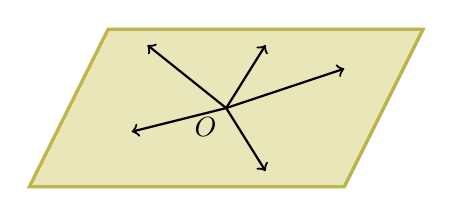
\begin{tikzpicture}
	% Параллелограмм
		\draw[draw = olive!60, fill = olive!20, very thick]
			(0,0) -- (4,0) -- (5,2) -- (1,2) -- cycle;
		% Центр параллелограмма O
		\coordinate (O) at (2.5,1);
		\point{O};
		\node[below left] at (O) {\(O\)};
		% Векторы из центра O
		\draw[->, thick] (O) -- ++(1.5,0.5);
		\draw[->, thick] (O) -- ++(-1,0.8);
		\draw[->, thick] (O) -- ++(0.5,-0.8);
		\draw[->, thick] (O) -- ++(-1.2,-0.3);
		\draw[->, thick] (O) -- ++(0.5,0.8);
	\end{tikzpicture}
	\end{adjustbox}\hfill
	\begin{adjustbox}{valign=t,minipage={0.62\textwidth}}
	\parbox{\linewidth}{
		$+:$ по правилу параллелограмма (так как векторы из одной точки)\\
		
	}
	\end{adjustbox}
	\end{figure}




\end{enumerate}

